\begin{frame}{Marco teórico - Problema de Kepler Newtoniano}
    Si $\vec{x}_1$ y $\vec{x}_2$ son las coordenadas de $m_1$ y $m_2$ respecto a un sistema de referencia
inercial, entonces las ecuaciones de movimiento correspondientes son:
\begin{equation}
\ddot{\vec{x}}_1=-Gm_2\frac{(\vec{x}_1-\vec{x}_2)}{|\vec{x}_1-\vec{x}_2|^3} ,\label{eq:acel1}
\end{equation}
\begin{equation}
\ddot{\vec{x}}_2=-Gm_1\frac{(\vec{x}_2-\vec{x}_1)}{|\vec{x}_1-\vec{x}_2|^3} .\label{eq:acel2}
\end{equation}
Es conveniente definir una coordenada para el centro de masa $\vec{x}_{cm}$, la cual esta dada por:
\begin{equation}
\vec{x}_{\rm cm}:=\frac{m_1\vec{x}_1+m_2\vec{x}_2}{M}, \qquad M:=m_1+m_2.
\end{equation}
\end{frame}
\begin{frame}{Marco teórico - Problema de Kepler Newtoniano}
    Con estas ecuaciones definidas se puede comprobar que a partir de \ref{eq:acel1} y \ref{eq:acel2}  el centro de masa $\vec{x}_{cm}$ es igual a cero.
    \begin{equation}
        \ddot{x}_{\rm cm} = \vec{0}.
        \label{eq:cm}
    \end{equation}
    Por la condición \ref{eq:cm} implica que, en el sistema de referencia inercial del centro de masa, las coordenadas
de $m_1$ y $m_2$ están relacionadas por:
\begin{equation}
    \vec{x}_2 = -\frac{m_1}{m_2} \vec{x}_1. \label{eq:x2x1}
\end{equation}
Definiendo así una coordenada relativa dada por:
\begin{equation}
    \vec{r}:= \vec{x}_2 - \vec{x}_1 \label{eq:r}.
\end{equation}
\end{frame}
\begin{frame}{Marco teórico - Problema de Kepler Newtoniano}
    Con esto definido, podemos escribir a la ecuación \ref{eq:x2x1} comprobar
\begin{equation}\label{eq:x12fr}
    \vec{x}_1=-\frac{m_2}{M}\vec{r}, \qquad \vec{x}_2=\frac{m_1}{M}\vec{r}.
\end{equation}
Usando estas relaciones podemos transformar las ecuaciones de movimiento \ref{eq:acel1} y \ref{eq:acel2} en ecuaciones para la coordenada relativa:
\begin{equation}
    \ddot{\vec{r}}=-GM \frac{\hat{r}}{r^2}.
    \label{eq:ddotr}
\end{equation}
Por otro lado, la energía total del sistema
\begin{equation}
    E=\frac{1}{2}m_1\vec{v}_1^2+\frac{1}{2}m_2\vec{v}_2^2-\frac{Gm_1m_2}{|\vec{x}_1-\vec{x}_2|},
\end{equation}
\end{frame}
\begin{frame}{Marco teórico - Problema de Kepler Newtoniano}
    y el momentum angular total respecto al origen,
\begin{equation}
    \vec{L}=m_1\vec{x}_1\times\vec{v}_1+m_2\vec{x}_2\times\vec{v}_2,
\end{equation}
    pueden reescribirse en términos de la coordenada relativa, resultando
\begin{equation}\label{eq:Er}
    E=\frac{1}{2}\mu \vec{v}^2-\frac{G\mu M}{r},
\end{equation}
\begin{equation}\label{eq:Lr}
    \vec{L}=\mu\,\vec{r}\times\vec{v},
\end{equation}
\end{frame}
\begin{frame}{Marco teórico - Problema de Kepler Newtoniano}
    \begin{align}
        \vec{v} & = \dot{r}\,\hat{r}+r\dot{\varphi}\,\hat{\varphi} ,\label{eq:vel1}\\
        \vec{a} & = \left(\ddot{r}-r\dot{\varphi}^2\right)\hat{r} +\left(r\ddot{\varphi}+2\dot{r}\dot{\varphi}\right)\hat{\varphi} .\label{eq:acer2}
    \end{align}
    Reemplazando la ecuación \ref{eq:acer2} en \ref{eq:ddotr} obtenemos
    \begin{eqnarray}
        \left(\ddot{r}-r\dot{\varphi}^2\right)\hat{r}+
        \left(r\ddot{\varphi}+2\dot{r}\dot{\varphi}\right)\hat{\varphi}
        =-\frac{GM}{r^2}\hat{r}.
    \end{eqnarray}
    De aqui, encontramos 
    \begin{eqnarray}
        \ddot{r}-r\dot{\varphi}^2&=&-\frac{GM}{r^2},\label{eq:acer3}\\
        r\ddot{\varphi}+2\dot{r}\dot{\varphi}&=&0.\label{eq:acer4}
    \end{eqnarray}
\end{frame}
\begin{frame}{Marco teórico - Problema de Kepler Newtoniano}
Multiplicando la ecuación \ref{eq:acer4} por r, se ecuentra que el término $r^2\phi$ es constante sobre la trayectoria
    \begin{eqnarray*}
        0&=&r^2\ddot{\varphi}+2r\dot{r}\dot{\varphi}\\
        &=&\frac{d}{dt}\left(r^2\dot{\varphi}\right),
    \end{eqnarray*}
    que expresa la conservación del momento angular, ya que
\begin{align*}
    \vec{L} & = \mu\,\vec{r}\times\vec{v}\\
    & = \mu\,r\,\hat{r}\times\left(\dot{r}\hat{r}+r\dot{\varphi}\hat{\varphi}
    \right)\\
    & = \mu\,r^2\dot{\varphi}\,(\hat{r}\times\hat{\varphi})\\
    & = \mu\,r^2\dot{\varphi}\,\hat{z}.
    \end{align*}
\end{frame}
\begin{frame}{Marco teórico - Problema de Kepler Newtoniano}
\begin{equation}
    \vec{L} = \mu\,r^2\dot{\varphi}\,\hat{z}. \label{eq:Ln}
\end{equation}
Otra cantidad conservada sobre la órbita es la energía mecánica
\begin{align}
    E&=\frac{1}{2}\mu v^2-\frac{GM\mu}{r} \label{eq:ener1}\\
    &=\frac{1}{2}\mu\dot{r}^2+\frac{1}{2}\mu r^2\dot{\varphi}^2-\frac{GM\mu}{r}.\label{eq:ener2}
\end{align}
Despejando $\dot{\varphi}$ de la ecuación \ref{eq:Ln} podemos escribir la energía mecánica sólo en términos de la variable r y constantes del movimiento:
\begin{eqnarray}
    E=\frac{1}{2}\mu\dot{r}^2+\frac{L^2}{2\mu r^2}-\frac{GM\mu}{r} .\label{eq:ener3}
\end{eqnarray}
\end{frame}
\begin{frame}{Marco teórico - Problema de Kepler Newtoniano}
    Definiendo un potencial efectivo
\begin{equation}
    V_{\rm ef}(r):=\frac{L^2}{2\mu r^2}-\frac{GM\mu}{r},
\end{equation}
De modo que la ecuación \ref{eq:ener3} pueda ser escrita como la ecuación de conservación de la energía de un movimiento unidimensional:
\begin{equation}
    E=\frac{1}{2}\mu\dot{r}^2+V_{\rm ef}(r) . \label{eq:EVef}
\end{equation}
    El potencial efectivo $V_{\rm ef}(r)$ posee un cero en
\begin{eqnarray}
    r_{\rm c}=\frac{L^2}{2GM\mu^2} ,\label{eq:cero1}
\end{eqnarray}
\end{frame}
\begin{frame}{Marco teórico - Problema de Kepler Newtoniano}
    \vspace{0.5cm}
    y además posee un mínimo en
    \begin{eqnarray}
    r_{\rm min}=\frac{L^2}{GM\mu^2}=2r_{\rm c},\label{eq:rmin}
    \end{eqnarray}
    tal que
    \begin{eqnarray*}
    V_{\rm ef, min}=-\frac{G^2M^2\mu^3}{2L^2}<0.
    \end{eqnarray*}
    Además, el comportamiento asintótico del potencial efectivo es
    \begin{eqnarray*}
    \lim_{r\to\infty}V_{\rm ef}(r)&\approx&-\frac{GMm}{r}\rightarrow 0,\\
    \lim_{r\to 0}V_{\rm ef}(r)&\approx&\frac{L^2}{2mr^2}\rightarrow +\infty .
    \end{eqnarray*} 
\end{frame}
\begin{frame}{Marco teórico - Problema de Kepler Newtoniano}
    \vspace{0.4cm}
    \begin{figure}[H]
        \centering
        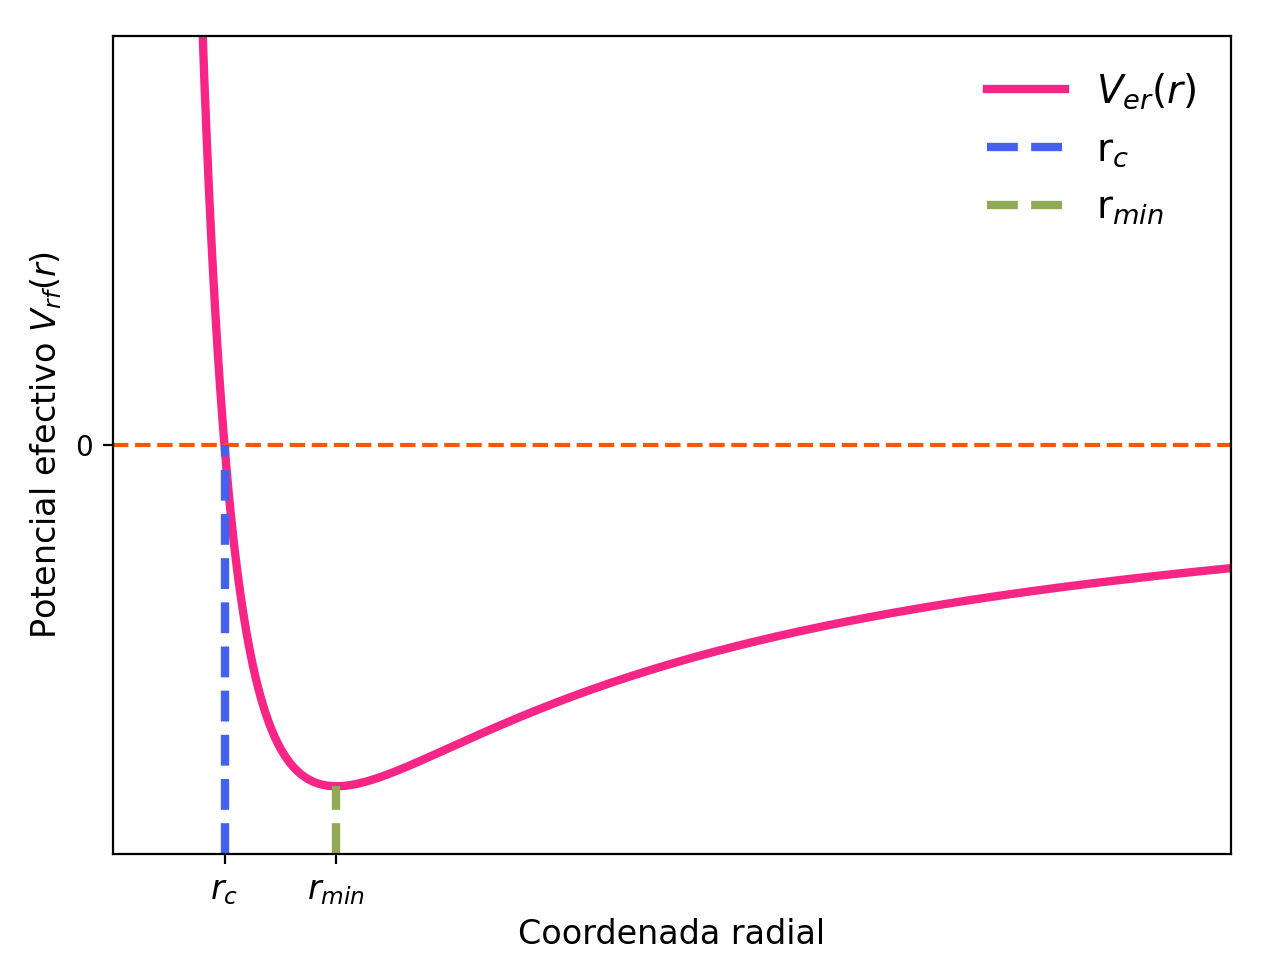
\includegraphics[scale=0.5]{images/Pot_efe.png}
        \caption{Potencial newtoniano efectivo, las constantes $L,G,M,\mu$ igualadas a 1}
        \label{fig:pot}
    \end{figure}
\end{frame}
\begin{frame}{Marco teórico - Problema de Kepler Newtoniano}
    Así para un valor de $L$ dado, tenemos que:
\begin{enumerate}
    \item Si $E_1>0$, una partícula proveniente del infinito alcanza un radio
    mínimo $r_1$, donde $\dot{r}^2=0$, y luego vuelve a infinito.
    \item Si $V_{\rm ef, min}<E_2<0$ la trayectoria es ligada, variando la distancia entre dos puntos de retorno $r_2$ y $r_3$, de modo que $r_2<r<r_{3}$.
    \item Si $E_{3}=V_{\rm ef, min}$ la partícula
    describe un movimiento circular de radio dado por la ecuación \ref{eq:rmin}. Este caso
    corresponde al mínimo del potencial, por lo que es un
    movimiento estable.
    \item Finalmente, no existen trayectorias con $E<V_{\rm ef, min}$ ya que la ecuación \ref{eq:EVef} requiere que $E\ge V_{\rm ef}$.
\end{enumerate}
\end{frame}
\begin{frame}{Marco teórico - Problema de Kepler Newtoniano}
\begin{eqnarray}
    \dot{r}=\frac{dr}{d\varphi}\dot{\varphi}=\frac{L}{\mu r^2}\frac{dr}{d\varphi}.
    \label{eq:dotr}
\end{eqnarray}
Reemplazando en la ecuación \ref{eq:ener3} la ecuación \ref{eq:dotr} obtenemos
\begin{equation}
    \frac{1}{r^4}\left(\frac{dr}{d\varphi}\right)^2=\frac{2\mu E}{L^2}+\frac{2GM\mu^2}{L^2r}-\frac{1}{r^2}.\label{eq:ener4}
\end{equation}
Con un cambio de variable $u:=1/r$, entonces la ecuación \ref{eq:ener4}
\begin{equation}
    (u')^2=\frac{2\mu E}{L^2}+\frac{2GM\mu^2}{L^2}\,u-u^{2
    },\label{eq:ener5}
    \end{equation}
derivando la ecuación \ref{eq:ener5} se encuentra la ecuación de movimiento para $u$ en funcion de $\varphi$
\begin{equation}
    u''+u=\frac{GM\mu^2}{L^2}.\label{eq:EC1}
\end{equation}
\end{frame}
\begin{frame}{Marco teórico - Problema de Kepler Newtoniano}
    La integración de la ecuación \ref{eq:EC1} es directa ya que corresponde a un oscilador armónico con un término forzante constante
\begin{equation}
    u(\varphi)=\frac{GM\mu^2}{L^2}\left(1+e\cos
    (\varphi-\varphi_0)\right)\label{eq:CON1}
\end{equation}
donde reemplazando la solución \ref{eq:CON1} en \ref{eq:ener5}
\begin{equation}
    e=\sqrt{1+\frac{2L^2E}{G^2M^2\mu^3}}, \label{eq:ex}
\end{equation}
\end{frame}
\begin{frame}{Marco teórico - Problema de Kepler Newtoniano}
    \vspace{0.3cm}
El semieje mayor de la órbita, puede ser escrito en términos de las constantes de movimiento a partir de las ecuaciones \ref{eq:CON1} y \ref{eq:ex}
\begin{align*}
    a & = \frac{1}{2}\left(\frac{1}{u_{\rm min}}+\frac{1}{u_{\rm max}}\right) \\
    & = \frac{1}{2}\left(\frac{L^2}{GM\mu^2}\frac{1}{(1+e)}+\frac{L^2}{GM\mu^2}\frac{1}{(1-e)}\right) \\
    & = \frac{L^2}{GM\mu^2}\frac{1}{(1-e^2)} \\
    & = -\frac{GM\mu}{2E}.
    \end{align*}
    \begin{equation}
        a= -\frac{GM\mu}{2E}. \label{eq:aE}
    \end{equation}
\end{frame}
\begin{frame}{Marco teórico - Problema de Kepler Newtoniano}
    Con esto, podemos escribir la solución de la ecuación \ref{eq:CON1} como 
\begin{equation}
    u(\varphi)=\frac{1}{a(1-e^2)}\left[1+e\cos
    (\varphi-\varphi_0)\right],
    \end{equation}
    o, en términos de la coordenada radial relativa,
    \begin{equation}\label{eq:rphi}
    r(\varphi)=\frac{a(1-e^2)}{1+e\cos(\varphi-\varphi_0)}.
\end{equation}
La evolución temporal de la órbita puede ser determinada implícitamente de la forma siguiente. Definamos la variable auxiliar
$s$ por
\begin{equation}\label{eq:rs}
    r:=a(1-e\cos s).
\end{equation}
\end{frame}
\begin{frame}{Marco teórico - Problema de Kepler Newtoniano}
    A partir de esto podemos usar la ecuación \ref{eq:rphi} para encontrar una relación entre $\varphi$ y $s$ sobre la órbita.
De esta forma, obtenemos 
\begin{equation}\label{eq:phiscos}
    \cos(\varphi-\varphi_0)=\frac{\cos s -e}{1-e\cos s},
\end{equation}
y a partir de aqui
\begin{equation}\label{eq:phissen}
    \sen(\varphi-\varphi_0)=\sqrt{1-e^2}\,\frac{\sen s}{1-e\cos s}.
\end{equation}
Derivando la ecuación \ref{eq:phiscos} respecto a $s$ y usando la ecuación \ref{eq:phissen} obtenemos 
\begin{equation*}
    \frac{d\varphi}{ds}=\frac{\sqrt{1-e^2}}{1-e\cos s}.
\end{equation*}
\end{frame}
\begin{frame}{Marco teórico - Problema de Kepler Newtoniano}
    \vspace{0.3cm}
    Con esto, podemos expresar el momento angular de la ecuación \ref{eq:Ln} en términos de $s$;
\begin{align*}
    L & = \mu r^2 \frac{d\varphi}{dt} \\
    & = \mu r^2 \frac{d\varphi}{ds}\frac{ds}{dt} \\
    & = \mu a^2\left(1-e\cos s\right)^2 \frac{d\varphi}{ds}\frac{ds}{dt} \\
    & = \mu a^2\sqrt{1-e^2}\left(1-e\cos s\right) \frac{ds}{dt} .
\end{align*}
Por lo tanto:
\begin{align*}
    1-e\cos s & = \frac{L}{\mu a^2\sqrt{1-e^2}} \frac{dt}{ds} \\
    & =: \omega_0 \frac{dt}{ds},
\end{align*}
\end{frame}
\begin{frame}{Marco teórico - Problema de Kepler Newtoniano}
    \begin{equation}
        1-e\cos s =: \omega_0 \frac{dt}{ds}, \label{eq:dtds}
    \end{equation}
    donde hemos introducido el término $\omega_0$, con unidades de frecuencia, que usando la ecuación \ref{eq:ex} satisface 
    \begin{equation}\label{eq:Kepler3}
        \omega_0^2=\frac{GM}{a^3}.    
    \end{equation}
\end{frame}
\begin{frame}{Marco teórico - Potencia radiada por un sistema binario}
    \begin{equation*}
        M_{ij}=m_1x_i^{(1)}x_{j}^{(1)}+m_2x_i^{(2)}x_{j}^{(2)}=\mu r_ir_j
    \end{equation*}
    Si las coordenadas son elegidas de modo que el movimiento del sistema está confinado al plano $xy$, tendremos que sólo $M_{11}$, $M_{12}$ y $M_{22}$ serán distintos de cero. De este modo, encontramos que
    \begin{align*}
    M_{11} & = \mu\, x^2\\
    & = \mu r^2\cos^2\varphi \\
    & = \mu a^2(1-e^2)^2\frac{\cos^2\varphi}{\left[1+e\cos(\varphi-\varphi_0)\right]^2},
    \end{align*}
\end{frame}
\begin{frame}{Marco teórico - Potencia radiada por un sistema binario}
    y, similarmente,
    \begin{align*}
    M_{12} & = \mu\, xy \\
    & = \mu r^2\cos\varphi\sen\varphi \\
    & = \mu a^2(1-e^2)^2\frac{\sen\varphi\cos\varphi}{\left[1+e\cos(\varphi-\varphi_0)\right]^2},
    \end{align*}
    \begin{align*}
    M_{22} & = \mu\, y^2 \\
    & = \mu r^2\sen^2\varphi \\
    & = \mu a^2(1-e^2)^2\frac{\sen^2\varphi}{\left[1+e\cos(\varphi-\varphi_0)\right]^2}.
    \end{align*}   
\end{frame}
\begin{frame}{Marco teórico - Potencia radiada por un sistema binario}
    A continuación requerimos determinar las terceras derivadas $\dddot{I}_{ij}$. Para esto, introducimos la coordenada angular $\varphi$ y usamos las ecuaciones \ref{eq:Ln} y \ref{eq:rphi}, de modo que podamos escribir
\begin{align*}
\dot{M}_{ij} &= \frac{dM_{ij}}{d\varphi}\dot{\varphi} \\
&= \frac{dM_{ij}}{d\varphi}\frac{L}{\mu r^2} \\
&= \frac{L}{\mu a^2(1-e^2)^2}\left[1+e\cos(\varphi-\varphi_0)\right]^2 \frac{dI_{ij}}{d\varphi}\\
&= \frac{\omega_0}{(1-e^2)^{3/2}}\left[1+e\cos(\varphi-\varphi_0)\right]^2 \frac{dI_{ij}}{d\varphi}.
\end{align*}
\end{frame}
\begin{frame}{Marco teórico - Potencia radiada por un sistema binario}
    Con lo que encontrariamos que 
\begin{equation*}
\dot{M}_{11}=(-2)\mu a^2\omega_0\left(1-e^2\right)^{1/2}\frac{\cos\varphi(\sen\varphi+e\sen\varphi_0)}{1+e\cos(\varphi-\varphi_0)},
\end{equation*}
\begin{equation*}
\dot{M}_{22}=(+2)\mu a^2\omega_0\left(1-e^2\right)^{1/2}\frac{\sen\varphi(\cos\varphi+e\cos\varphi_0)}{1+e\cos(\varphi-\varphi_0)},
\end{equation*}
\begin{equation*}
    \dot{M}_{12}=\mu a^2\omega_0\left(1-e^2\right)^{1/2}\frac{(\cos2\varphi+e\cos(\varphi+\varphi_0))}{1+e\cos(\varphi-\varphi_0)}.
\end{equation*}
\end{frame}
\begin{frame}{Marco teórico - Potencia radiada por un sistema binario}
Análogamente, encontramos que
\begin{equation}\label{eq:I11}
    \changefontsizes{9pt}
\dddot{M}_{11}=\alpha\left[1+e\cos(\varphi-\varphi_0)\right]^2 \left[4\sen(2\varphi)+3e\sen(2\varphi)\cos(\varphi-\varphi_0)
+2e\cos\varphi\sen\varphi_0\right],
\end{equation}
\begin{equation}\label{eq:I22}
    \changefontsizes{9pt}
\dddot{M}_{22}=\alpha\left[1+e\cos(\varphi-\varphi_0)\right]^2 \left[-4\sen(2\varphi)-3e\sen(2\varphi)\cos(\varphi-\varphi_0)
-2e\sen\varphi\cos\varphi_0\right],
\end{equation}
\begin{equation}\label{eq:I12}
    \changefontsizes{9pt}
\dddot{M}_{12}=\alpha\left[1+e\cos(\varphi-\varphi_0)\right]^2 \left[-4\cos(2\varphi)-3e\cos(2\varphi)\cos(\varphi-\varphi_0)
-e\cos(\varphi+\varphi_0)\right],
\end{equation}
con
\begin{equation*}
\alpha:=\frac{\mu a^2\omega_0^3}{\left(1-e^2\right)^{5/2}}.
\end{equation*}
\end{frame}
\begin{frame}{Marco teórico - Potencia radiada por un sistema binario}
    En términos del tensor momento de inercia con traza, la potencia promedio radiada se reduce en este caso a
\begin{align*}
\left\langle P\right\rangle &=\frac{G}{5c^5}\, \left\langle \dddot{M}^{ij}\dddot{M}^{ij}-\frac{1}{3}\left(\dddot{M}^{ii}\right)^2\right\rangle \\
&=\frac{G}{5c^5}\, \left\langle \left(\dddot{M}_{11}\right)^2+ \left(\dddot{M}_{22}\right)^2+2 \left(\dddot{M}_{12}\right)^2-\frac{1}{3}\left(\dddot{M}_{11}+\dddot{M}_{22}\right)^2\right\rangle \\
&=\frac{2G}{15c^5}\, \left\langle \left(\dddot{M}_{11}\right)^2+ \left(\dddot{M}_{22}\right)^2+3\left(\dddot{M}_{12}\right)^2 -\dddot{M}_{11}\dddot{M}_{22}\right\rangle .
\end{align*}
Luego de reemplazar las ecuaciones \ref{eq:I11} y \ref{eq:I12}, y usando la ecuación \ref{eq:Kepler3}, obtenemos
\begin{equation*}
\left\langle P\right\rangle = \frac{2G^4\mu^2M^3}{15c^5a^5\left(1-e^2\right)^{5}}\left\langle g(\varphi)\right\rangle ,
\end{equation*}
\end{frame}
\begin{frame}{Marco teórico - Potencia radiada por un sistema binario}
donde hemos introducido la función angular
\begin{equation}\label{eq:Pphi}
    \changefontsizes{10pt}
g(\varphi):=2\left[1+e\cos(\varphi-\varphi_0)\right]^4
\left[24+13e^2+48e\cos(\varphi-\varphi_0) +11e^2\cos(2\varphi-2\varphi_0)\right].
\end{equation}
\end{frame}
\begin{frame}{Marco teórico - Potencia radiada por un sistema binario}
Para calcular el promedio $\left\langle g(\varphi)\right\rangle$, transformamos la integral temporal en una integral sobre el ángulo $\varphi$:
\begin{align*}
\left\langle g(\varphi)\right\rangle &= \frac{1}{T}\int_0^T g(t)\,dt \\
&= \frac{1}{T}\int_0^{2\pi} g(\varphi)\frac{dt}{d\varphi}\,d\varphi \\
&= \frac{1}{T}\frac{\mu}{L}\int_0^{2\pi} r^2(\varphi)g(\varphi)\,d\varphi \\
&= \frac{(1-e^2)^{3/2}}{2\pi}\int_0^{2\pi} \frac{g(\varphi)}{\left[1+e\cos(\varphi-\varphi_0)\right]^2}\,d\varphi.
\end{align*}
\end{frame}
\begin{frame}{Marco teórico - Potencia radiada por un sistema binario}
Luego de reemplazar \ref{eq:Pphi} en la expresión anterior, se obtiene una integral de simples funciones trigonométricas, que al ser evaluada se reduce a
\begin{equation*}
    \left\langle g(\varphi)\right\rangle= 48(1-e^2)^{3/2}\left(1+\frac{73}{24}e^2+\frac{37}{96}e^4\right).
    \end{equation*}
    Con esto, encontramos la expresión de la potencia total promedio radiada por un sistema binario, de masa total $M$, masa reducida $\mu$, describiendo una órbita (relativa) con semieje mayor $a$, y excentricidad $e$ \cite{PhysRev.131.435}.
    \begin{equation}\label{eq:PSbin}
    \left\langle P\right\rangle =\frac{32}{5}\frac{G^4\mu^2M^3}{c^5a^5}\,f(e),
    \end{equation}
\end{frame}
\begin{frame}{Marco teórico - Potencia radiada por un sistema binario}
    \begin{equation*}
        f(e):=\frac{1}{\left(1-e^2\right)^{7/2}}\left(1+\frac{73}{24}e^2+\frac{37}{96}e^4\right).
        \end{equation*}
        Análogamente, el momentum angular promedio radiado es
        \begin{equation*}
        \langle\dot{L}\rangle=\frac{32}{5}\frac{G^{7/2}\mu^{2}M^{5/2}}{c^5a^{7/2}}\frac{1}{(1-e^{2})^{2}}\left[1+\displaystyle\frac{7}{8}e^{2}\right].
        \end{equation*}
\end{frame}
\begin{frame}{Marco teórico - Potencia radiada por un sistema binario}
De aquí encontramos la predicción de la \textit{Teoría de Relatividad General para la disminución del periodo orbital de un sistema binario debido a la emisión de radiación gravitacional}:
\begin{align*}
\frac{\dot{T}}{T} &= -\frac{3}{2}\frac{\dot{E}}{E} \\
&= -\frac{96}{5} \frac{G^{5/3}\mu M^{2/3}}{c^5}\left(\frac{T}{2\pi}\right)^{-8/3}f(e).
\end{align*}
\vspace{-0.7cm}
\begin{align}
\frac{da}{dt} &= -\frac{64}{5}\frac{G^3\mu M^2}{c^5a^3}\frac{1}{\left(1-e^2\right)^{7/2}}\left(1+\frac{73}{24}e^2+\frac{37}{96}e^4\right) \label{eq:dadt},\\
\frac{de}{dt} &= -\frac{304}{15}\frac{G^3\mu M^2}{c^5a^4}\frac{e}{\left(1-e^2\right)^{5/2}}\left(1+\frac{121}{304}e^2\right). \label{eq:dedt}
\end{align}
\end{frame}
\begin{frame}{Marco teórico - Potencia radiada por un sistema binario}
En el caso de una órbita circular, $e=0$, la ecuación se reduce a
\begin{equation}
\frac{da}{dt} = -\frac{64}{5}\frac{G^3\mu M^2}{c^5a^3},
\end{equation}
cuya solución es
\begin{equation}
a(t) = \left[a_0^4-\frac{256}{5}\frac{G^3\mu M^2}{c^5}(t-t_0)\right]^{1/4}.
\end{equation}
\end{frame}
\begin{frame}{Marco teórico - Potencia radiada por un sistema binario}
Dividiendo las ecuaciones \ref{eq:dadt} y \ref{eq:dedt} para $\dot{a}$ y $\dot{e}$ podemos eliminar el tiempo de estas expresiones y encontrar una ecuación que relaciona directamente $a$ con $e$:
\begin{equation}
\frac{da}{de}=\frac{12}{19}a\frac{1+(73/24)e^2+(37/96)e^4}{e(1-e^2)[1+(121/304)e^2]}.
\label{eq:dade}
\end{equation}
La solución de esta ecuación es de la forma
\begin{equation*}
a(e)=a_{0}\frac{g(e)}{g(e_{0})},
\end{equation*}
con 
\begin{equation*}
g(e):= \frac{e^{12/19}}{1-e^2}\left(1+\frac{121}{304} \right)^{870/2299}.
\end{equation*}
\end{frame}